\cleartooddpage[\thispagestyle{empty}]
\chapter{Analysis}

\section{Studies}
Backgrounds from data were analyzed.

\subsection{Effect of Stars}
To examine the effect of stars on the camera, several studies were undertaken.
It had been noted in the past that for a dim star (magnitude > 5??), the given pixel would have a higher average current.
This translated into a higher pedvar??, which can contribute to images, under certain conditions??.

In addition, if a bright star (magnitude <= 5??) was in the field of view, it would cause such a high current in the pixel that it would have to be shut off (voltage set to 0??) to prevent it from being damaged.
For particularly bright stars (magnitude <= 3), often several pixels would be disabled at a given time.

A third effect is that, since the telescope camera is fixed to the ground, from the camera's point of view the sky rotates around the camera center.
This means that over a single 30min observation, any stars rotate around the camera center, disabling several camera pixels as it passes over them.

This implies a key idea, that to study the effect of stars, one should study the effect of high-current or disabled camera pixels, and use this information to construct the effect of stars.

% see calculations/disabledpixel_obstime , those 250 crab runs turned into about 13.5 observation hours
To examine the effects of disable pixels, a study was performed where 13.5 hours of Crab observations were analyzed twice, once normally, and once with a single pixel disabled in all four telescopes.
This mimics the effect of having a star in the field of view that is bright enough to disable a pixel.
Once the events are reconstructed, and passed through gamma-hadron cuts, they can then be compared.
When synchronizing the event lists, it can be done in $O\left(n\right)$ time, as both event lists are already time-ordered.
After the event lists with the pixel enabled and disabled are synchronized, they can be compared.
One can then look for events that disappeared when the pixel was disabled, as well looking for new events that appeared.
Events that are still present in both event lists can then be tested to see how far their reconstructed camera position moved.


\begin{figure}[h]\label{fig:dpix_rel_camera}
  \begin{center}
    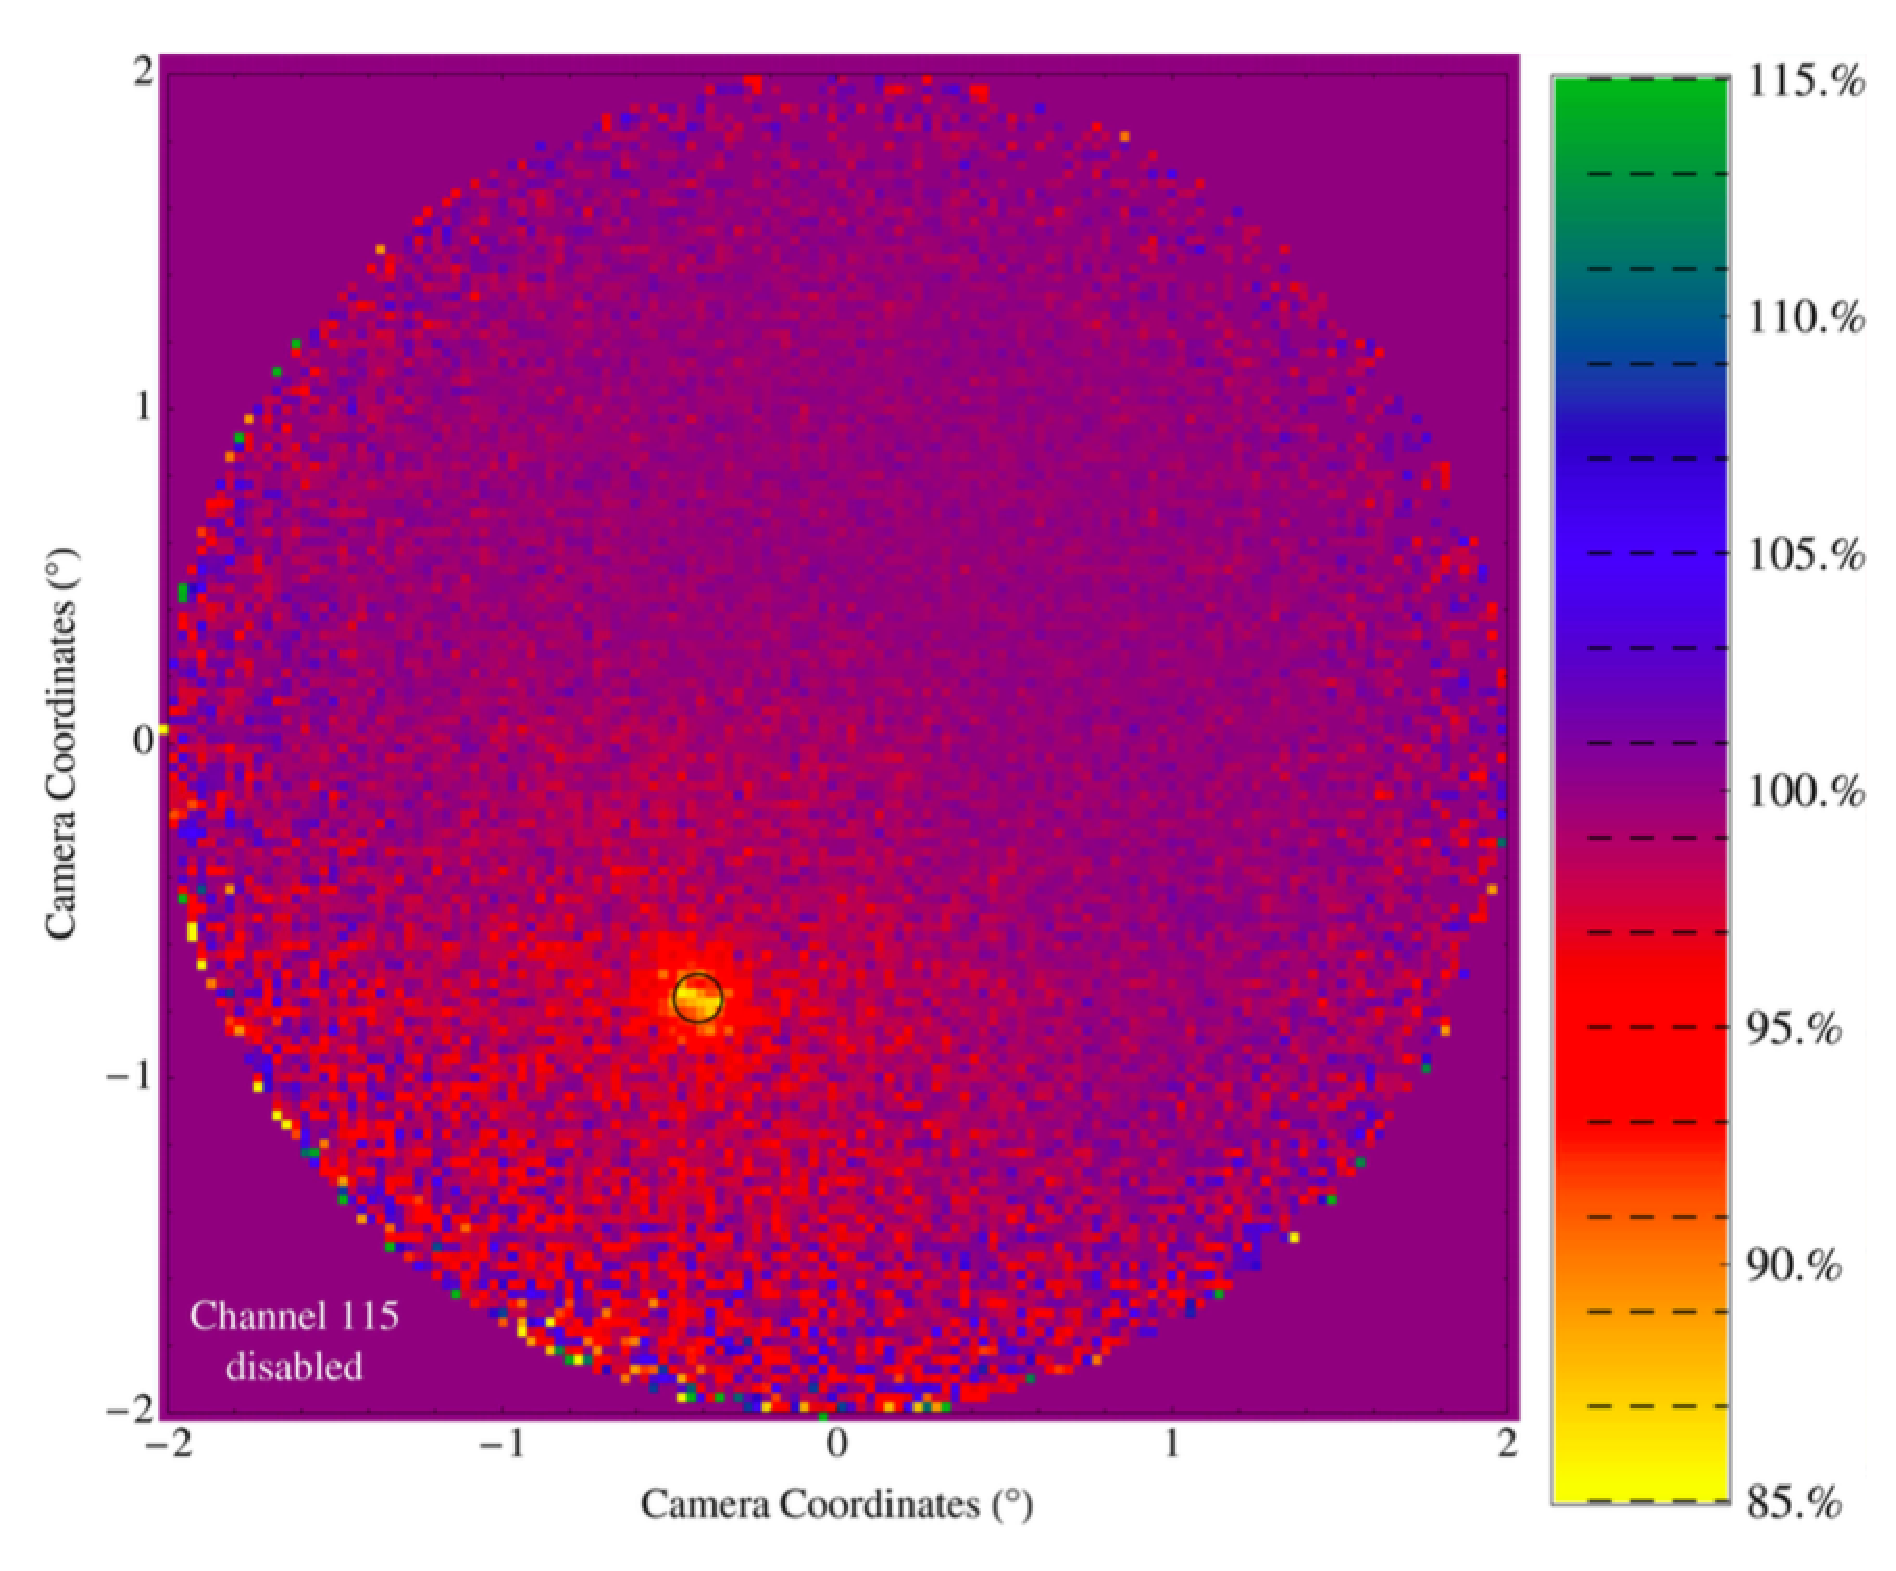
\includegraphics[width=0.8\textwidth]{images/disabled_pixel/relativerate_camera}
    \caption[Relative Event Rate]{Event rate in the camera with pixel 115 disabled in all four telescopes, relative to having all pixels enabled.  Camera coordinate axes are parallel to azimuth and elevation.}
  \end{center}
\end{figure}

\begin{figure}[h]\label{fig:dpix_rel_radial}
  \begin{center}
    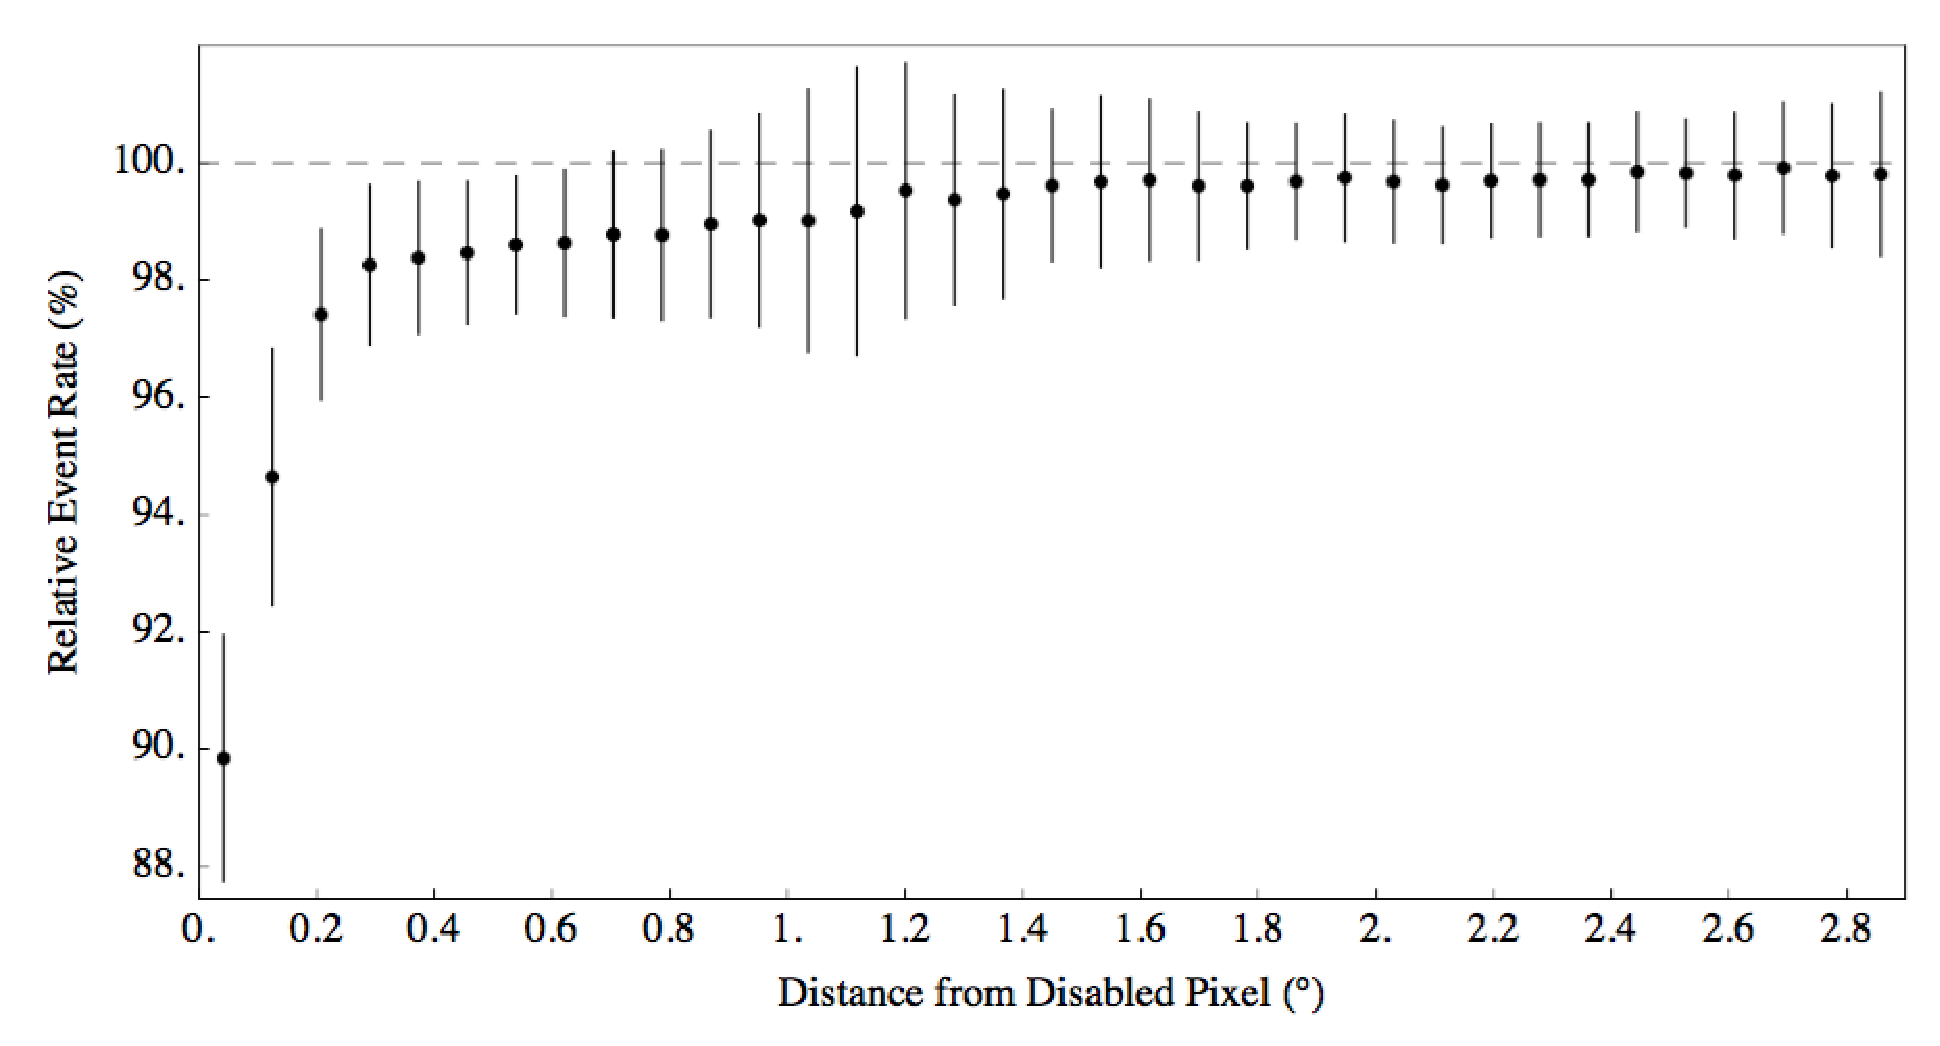
\includegraphics[width=\textwidth]{images/disabled_pixel/relativerate_radial}
    \caption[Radial Relative Event Rate]{Same relative event rate as in figure \ref{fig:dpix_rel_camera}, but averaged into radial bins, centered on the disabled pixel 115. }
  \end{center}
\end{figure}

\begin{figure}[h]\label{fig:dpix_disappear}
  \begin{center}
    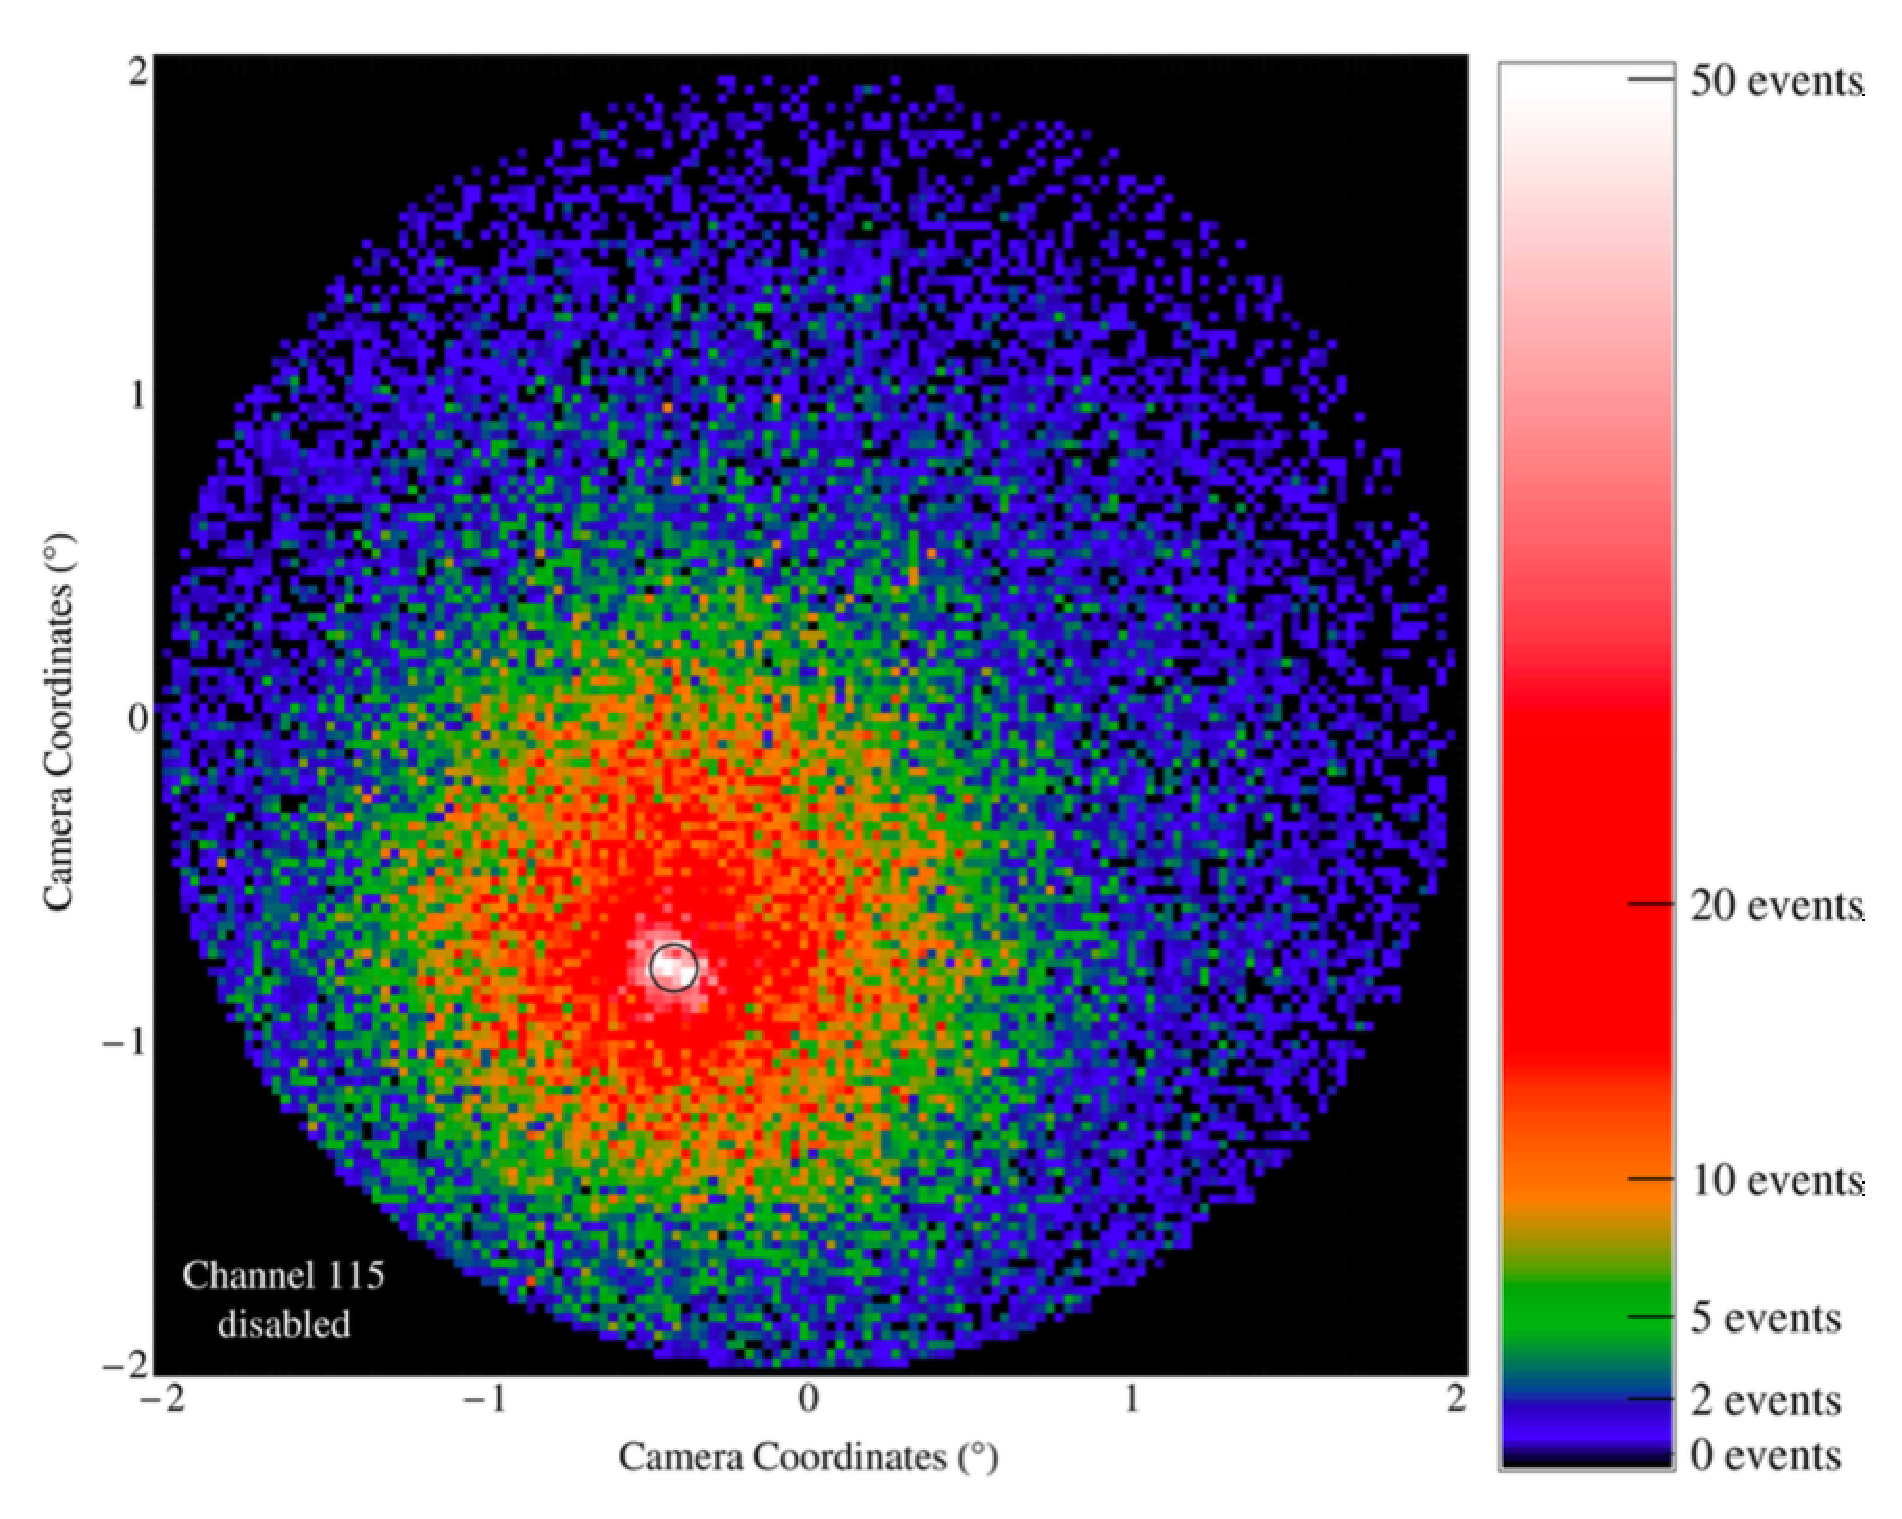
\includegraphics[width=0.8\textwidth]{images/disabled_pixel/disappearing_events}
    \caption[Disappering Events]{Positions of events that disappeared when pixel 115 was disabled in all four telescopes.  Positions are from their pixel-enabled reconstructed position.}
  \end{center}
\end{figure}

\begin{figure}[h]\label{fig:dpix_appear}
  \begin{center}
    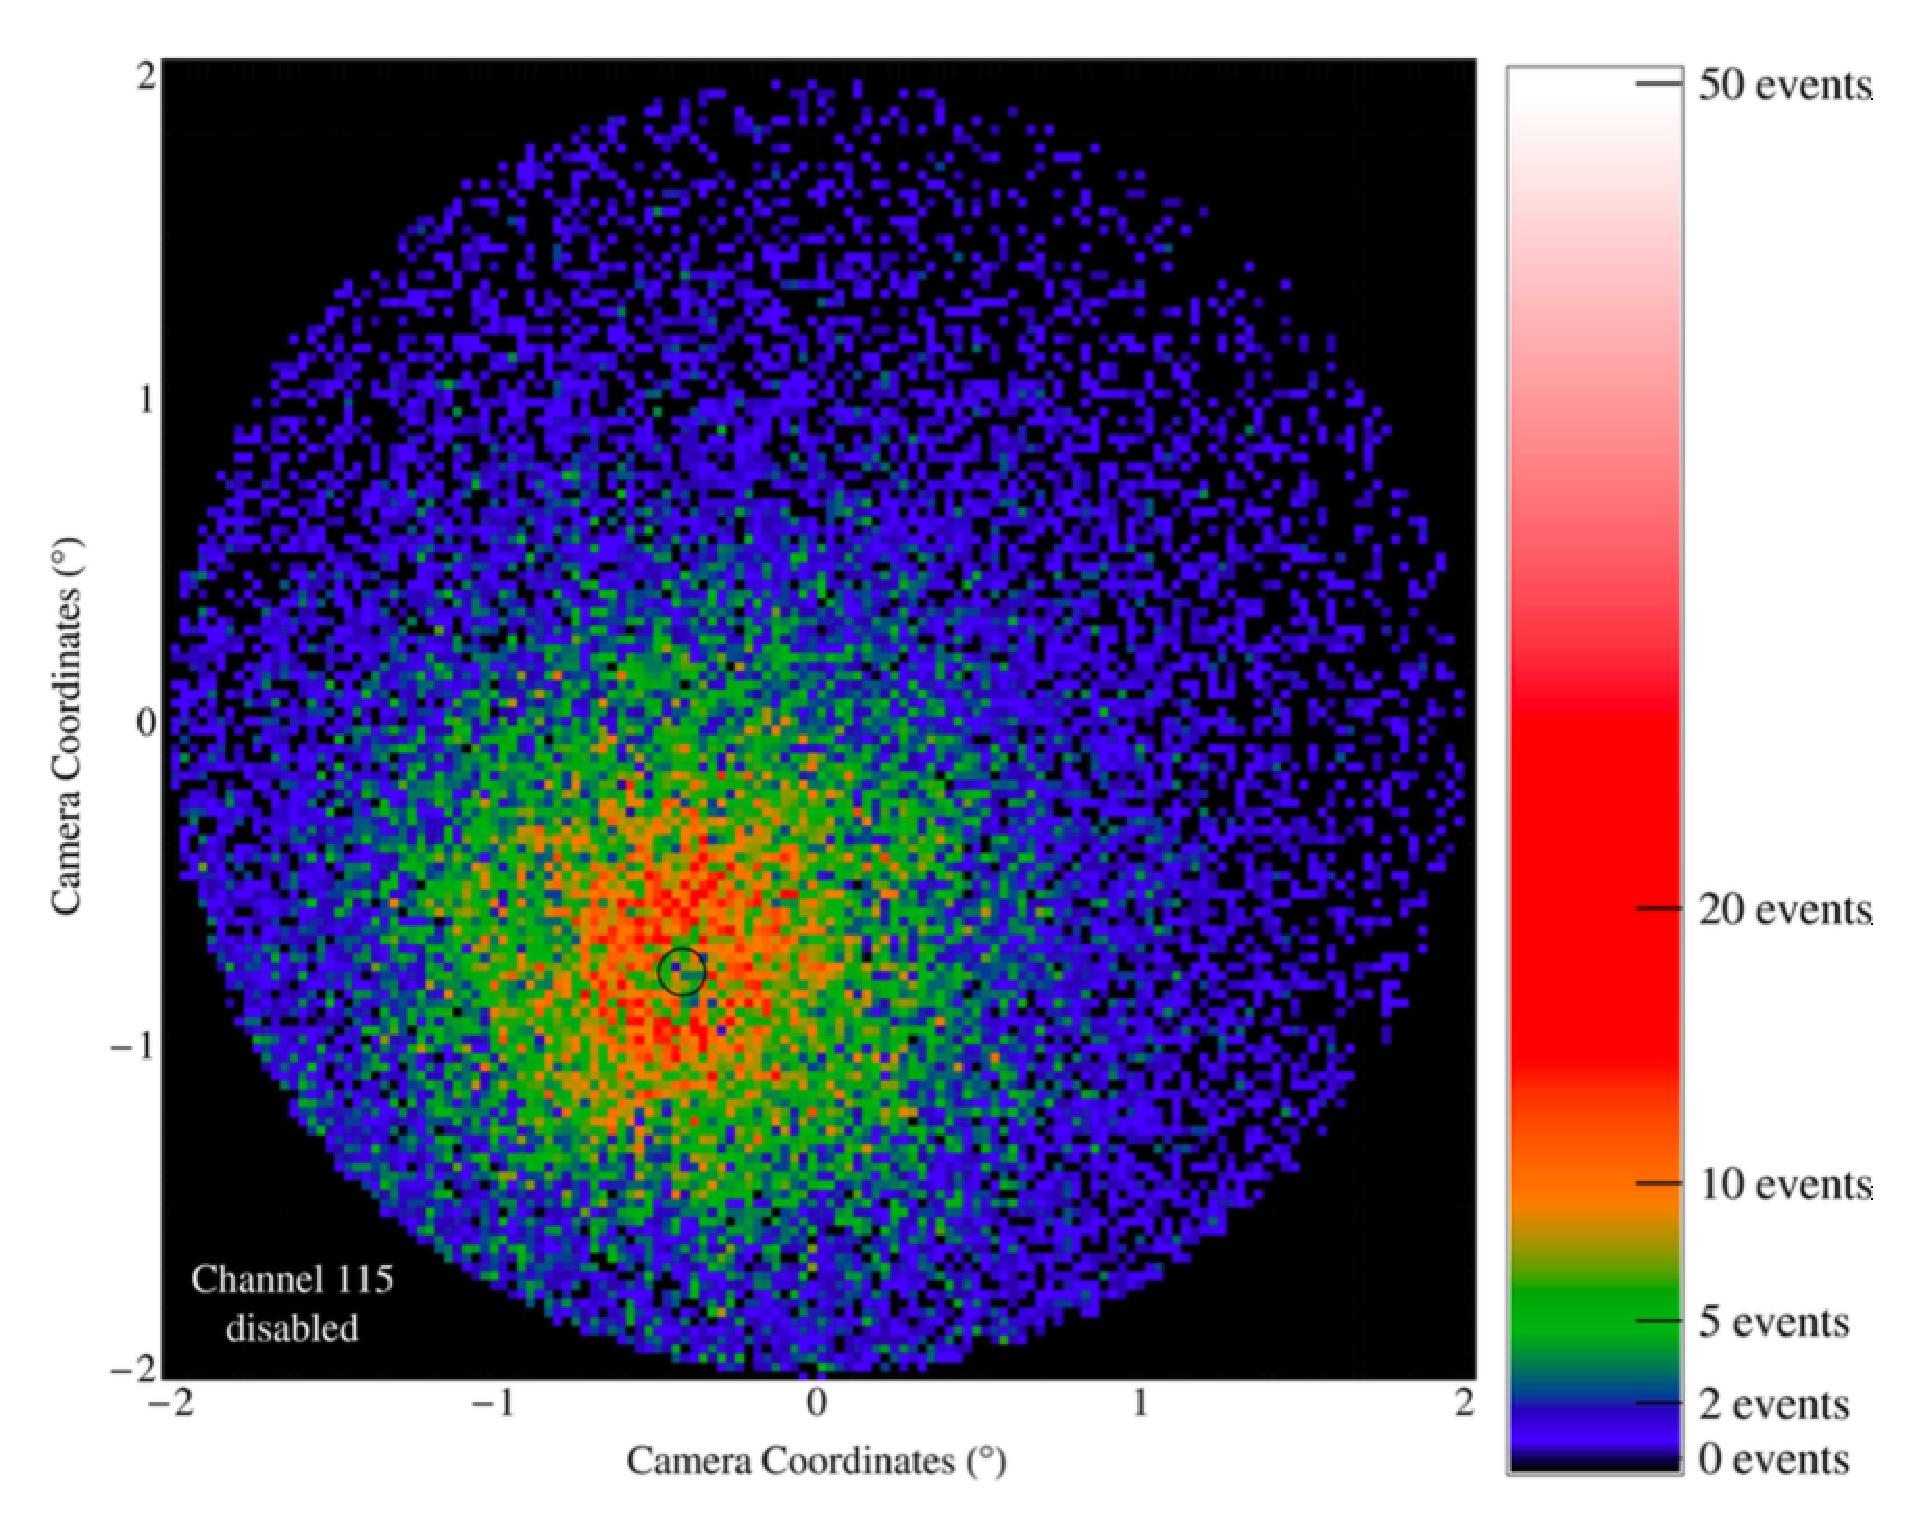
\includegraphics[width=0.8\textwidth]{images/disabled_pixel/appearing_events}
    \caption[Newly Appearing Events]{Positions of new events that appeared when pixel 115 was disabled in all four telescopes.  Positions are from their pixel-disabled reconstructed position.  It should be noted that these are not completely new events.  They are only new events in that, due to the pixel being disabled, they now pass cuts that they previously failed.}
  \end{center}
\end{figure}

\begin{figure}[h]\label{fig:dpix_move}
  \begin{center}
    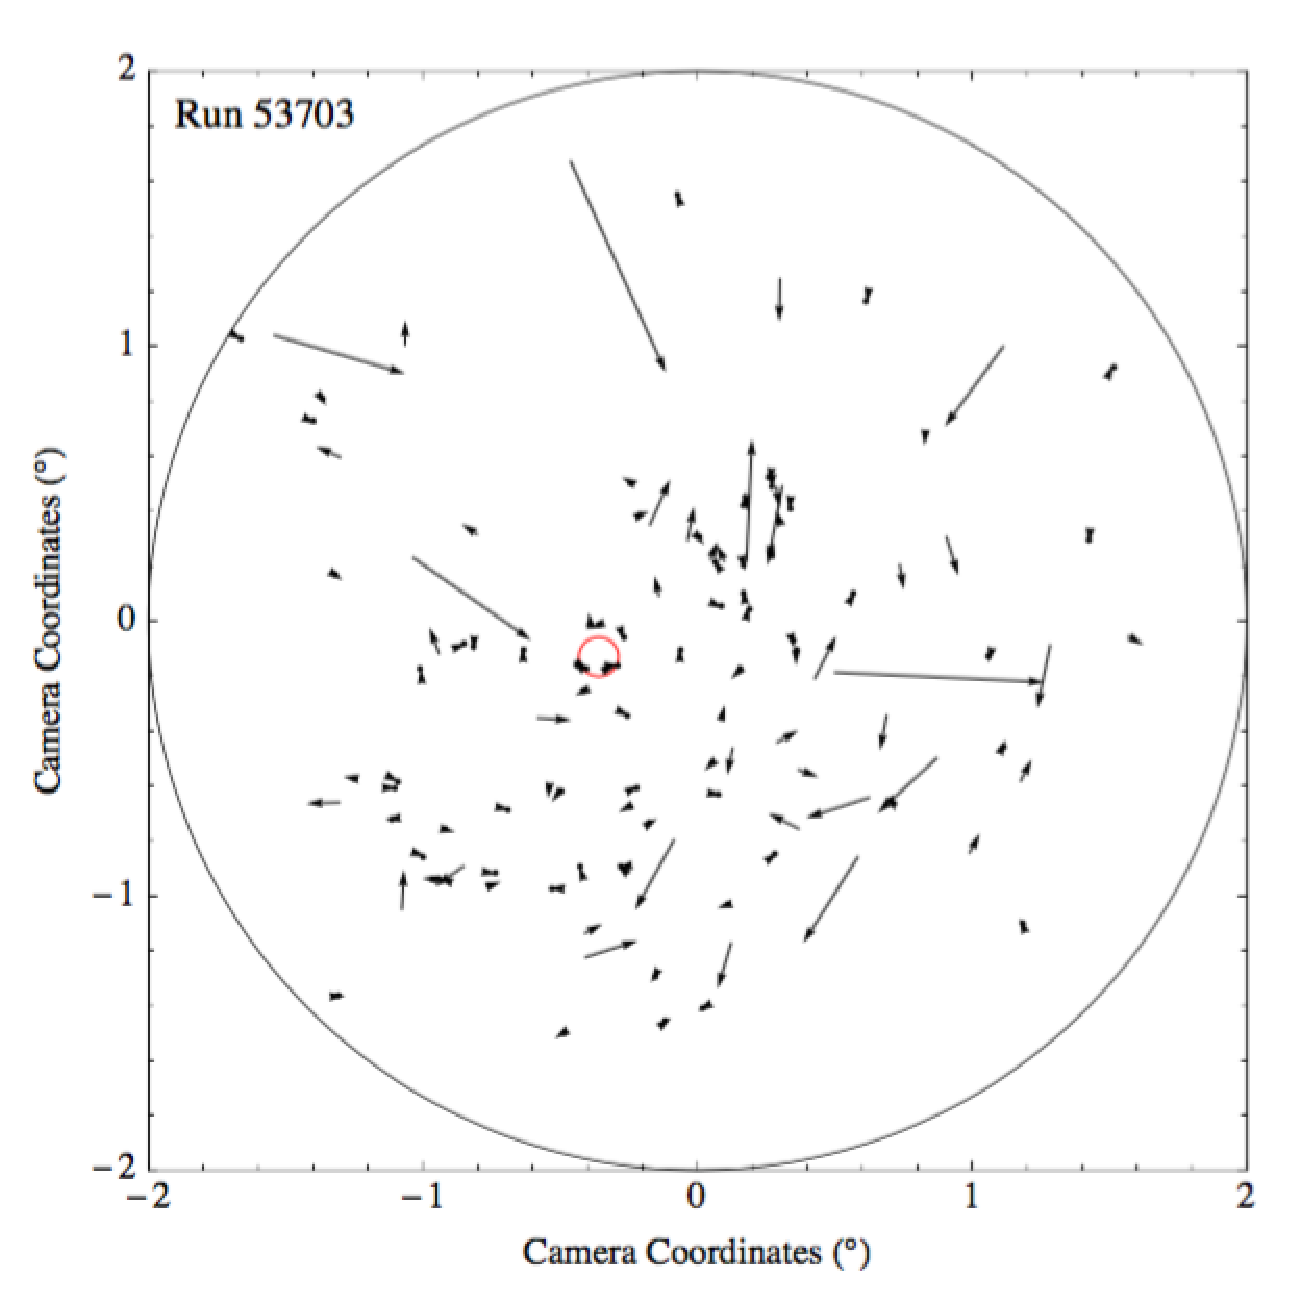
\includegraphics[width=0.8\textwidth]{images/disabled_pixel/moving_events}
    \caption[Event Movement]{Positions of events that moved when pixel 115 (denoted by the red circle) was disabled in all four telescopes.  Arrow points from the pixel-enabled position to the pixel-disabled position.  Only events that moved more that 0.1*PSF are shown.}
  \end{center}
\end{figure}


\subsection{Low Elevations}
For VERITAS, the galactic center is at a low elevation, usually around 29 degrees.
As part of the observing strategy for the galactic center, off data is also taken near the galactic center.
This means that, for most nights when the galactic center is observed (called On runs, at RA/Dec 260.91/-29.01), one run is also taken with the observatory pointing a few degrees away from the galactic center, an Off run at RA/Dec 266.41/-29.01 .
This is done because the galactic center is a highly active area, meaning there are few regions within the On data that can be used as a background region in the Li and Ma significance equation ??.

Data in two different elevation brackets.

Shows Crescent pattern at lowest energies, doughnut at slightly higher energies, then at higher energies is concentrated at the lower part of the camera.

\subsection{Diffuse Gamma Rays}

Sets gamma rays were simulated, with corsika, at different energies.
These gamma rays were diffused in a circular disk of radius ?? degrees around ?? elevation/azimuth.
The gamma rays were then processed through the VERITAS simulation chain.
This simulation chain takes the cherenkov photons from each gamma ray shower, and calculates which ones hit telescope mirrors.
Then, it calculates which cherenkov photons hit which pixels, and at what time.
Once cherenkov photons are measured hitting a pixel, a hardware simulation program takes over to simulate the voltage pulse created by the photons.
This voltage pulse is then propagated through a software simulation of the VERITAS triggering system.
Once the list of triggered gamma-ray showers is save to a file, reconstruction of the event can be done by the same software that reconstructs observed events.

\subsection{Elevation Effects}

Diffuse sims with direct-camera pointing show just the elevation effects, no camera effects.
To study the effect of elevation, special diffuse sims were made.
These were produced such that, after creating diffuse gamma rays in corsika, the simulated telescopes were pointed directly at each event.
This means that while the events were at a variety of azimuths and elevations, they all hit in the center of the camera.

From these plots, one can see that different gamma-ray energies have different horizon elevations, below which a particular energy gamma ray cannot be detected.

By looking at the number of gamma rays detected at each energy and elevation (and ignoring azimuth), the slope of the elevation effect can be seen.
It is important to note, that each energy has a different slope due to elevation.


\subsection{Gamma Verses Protons}

Doughnut shapes appear in the gamma-like protons.


\section{Veritas Data}
runs/sources/dates/times

\section{Likelihood Ratio Test}
The likelihood ratio test useful for comparing two hypotheses.
They are referred to as the null and alternative hypotheses.
Each hypothesis consists of a predicted number of events at each point in the energy/space/time parameter space.
Once each hypothesis is constructed, the likelihood for each can be computed.
The ratio of the two likelihoods then follows a gaussian (with certain assumptions), meaning the sigificance of the alternative hypothesis over the null can be calculated.

\section{Backgrounds}

Backgrounds were from data.

\section{Test Sources}

  \subsection{Crab}
    Only studied runs with elevations between 70 and 75 degrees.
    Used Segue 1 data at the same elevations as a background.

    \subsubsection{Event Display}
    \subsubsection{CTOOLs}

  \subsection{HESS J0632 +057}
    Only studied data with pointing elevations between 59 and 65 degrees.
    Used Draco data at the same elevations as the background.

    \subsubsection{Event Display}
    \subsubsection{CTOOLs}

  \subsection{1ES 0414+009}
    Only studied data with pointing elevations between 53 and 60 degrees.
    Used Ursa Major II data at the same elevations as the background.

    \subsubsection{Event Display}
    \subsubsection{CTOOLs}

  \subsection{1ES1959+650}
    Only studied data with pointing elevations between 50 and 55 degrees.
    Used Ursa Minor data at the same elevations as the background.

    \subsubsection{Event Display}
    \subsubsection{CTOOLs}

\section{Sgr A* Data Analysis}
Broke data into two elevation regimes, 25-28.5 degrees, and 28.5 to 30.25 degrees.
Separate off runs were taken to use as a background.

  \subsubsection{Event Display}

\section{Astrophysical Models}

\subsection{Point Sources}

\subsection{Supernovas}

\subsection{Diffuse Emission}

\subsection{Dark Matter}

\section{Upper Limit}

comparison to 

